\documentclass[conference]{IEEEtran}
\IEEEoverridecommandlockouts
\usepackage[T1]{fontenc}
\usepackage{cite}
\usepackage{amsmath,amssymb,amsfonts}
\usepackage{graphicx}
\usepackage{algorithm}
\usepackage{algorithmic}
\usepackage{textcomp}
\usepackage{xcolor}
\usepackage{balance}
\usepackage{multirow}
\usepackage{booktabs}
\usepackage{caption}
\usepackage{subfig}
\usepackage{hyperref}
\hypersetup{hidelinks}
\usepackage{tikz}
\usetikzlibrary{positioning, arrows.meta, shapes.geometric, fit, calc, shadows}

\def\BibTeX{{\rm B\kern-.05em{\sc i\kern-.025em b}\kern-.08em
    T\kern-.1667em\lower.7ex\hbox{E}\kern-.125emX}}

\pagestyle{plain}

\begin{document}

\title{Securing IoT Transit: A Measurement Study of\\Practical Post-Quantum Gateway Translation}

\author{\IEEEauthorblockN{Sheikh Sayed Bin Rahman, Wan Nursyafeeza Binti Wan Mohd Nasir, Kanita Jerin Tanha, Minsoo Kim, and Taesoo Jun}
\IEEEauthorblockA{Pervasive Intelligent Computing Laboratory, Department of IT Convergence Engineering\\
Kumoh National Institute of Technology, Gumi, South Korea\\
Email: (sksayed, syafeeza, kanitajerin17, kms991022, taesoo.jun)@kumoh.ac.kr}}

\maketitle

\begin{abstract}
IoT gateways aggregate device-to-cloud MQTT traffic yet are rarely treated as a cryptographic upgrade boundary. We propose a transparent post-quantum pipeline where the gateway decrypts incoming MQTT messages and re-encrypts the plaintext with ML-KEM-768 and ML-DSA-65 (NIST Level~3, FIPS~203/204) before cloud forwarding, leaving device firmware unmodified. Evaluated on a Raspberry Pi~4B with real liboqs primitives across 1,000 messages with 5~KB payloads, the pipeline achieves a mean overhead of \textbf{0.189~ms} (P95: 0.297~ms). PQC primitives introduce a fixed 4,425-byte overhead per message, expanding a 5~KB payload to 9.4~KB; by confining this to the high-capacity uplink, the architecture is viable for production IoT deployments.
\end{abstract}

\begin{IEEEkeywords}
Post-Quantum Cryptography, ML-KEM-768, ML-DSA-65, MQTT, IoT Gateway, liboqs, Raspberry Pi
\end{IEEEkeywords}

\noindent\textbf{Acronyms:} PQC--Post-Quantum Cryptography; ML-KEM--Module-Lattice KEM (FIPS~203); ML-DSA--Module-Lattice DSA (FIPS~204); HNDL--Harvest-Now-Decrypt-Later; MQTT--Message Queuing Telemetry Transport.

\section{Introduction}

The IoT ecosystem faces a compounding cryptographic crisis. Shor's algorithm~\cite{shor1994} breaks RSA and ECC key exchange in polynomial time, while harvest-now-decrypt-later (HNDL) adversaries archive ciphertext today for future quantum decryption~\cite{mosca2018}. NIST finalized ML-KEM~\cite{nist_fips203} and ML-DSA~\cite{nist_fips204} as the first PQC standards in 2024, but deploying them on constrained IoT endpoints ($<$50~KB RAM) is often infeasible due to their larger key and signature sizes.

MQTT concentrates risk at the broker: most deployments protect the device-to-broker segment with AES (quantum-safe under Grover) while leaving the broker-to-cloud segment on classical TLS, creating a structural vulnerability for HNDL adversaries. Prior work integrates PQC into TLS~1.3 or proxy re-encryption schemes, but lacks empirical validation on commodity edge hardware. We treat the gateway as an application-layer translation point and provide the first measured latency and bandwidth characterization of this approach on real ARM hardware.

\textbf{Contributions.} We implement an MQTT gateway pipeline that (1)~decrypts device messages, (2)~re-encrypts the plaintext with ML-KEM-768 + AES-256-GCM + ML-DSA-65, and (3)~publishes to the cloud without any firmware changes on the IoT devices. We evaluate on a Raspberry Pi~4B with genuine liboqs primitives, measuring nanosecond-precision per-stage latency and quantifying the resulting bandwidth overhead across 1,000 live messages.

\section{Proposed Gateway Translation}

\subsection{Architecture and Threat Model}

Figure~\ref{fig:pipeline} shows the pipeline. IoT clients publish JSON payloads to a Mosquitto MQTT broker; the gateway subscribes, translates each payload to PQC-protected form, and republishes to the cloud consumer. We consider a passive HNDL adversary on the gateway-to-cloud link. Replay protection is enforced via per-session monotonic sequence numbers. A fresh ML-KEM encapsulation per message provides post-quantum forward secrecy on the uplink; the device-to-gateway link uses static AES-256, inherently resistant to Grover's algorithm.

Key pairs are provisioned out-of-band: the cloud generates an ML-KEM-768 keypair and shares only $pk_\text{cloud}$ with the gateway; the gateway generates an ML-DSA-65 keypair and shares only $pk_\text{gw}$ with the cloud. Private keys never leave their respective environments. In our prototype the pipeline runs in userspace; production deployments should isolate it within a hardware-backed TEE such as ARM TrustZone.

ML-KEM-768 provides IND-CCA2 confidentiality (NIST Level~3), with a fresh encapsulation per message ensuring post-quantum forward secrecy. ML-DSA-65 provides EUF-CMA authenticity; the signature covers the full tuple $(c_\text{kem}, c_\text{aes}, \eta)$, preventing substitution attacks. The device-to-gateway link uses static AES-256 (quantum-safe under Grover) but without forward secrecy, a limitation acknowledged for future work.

\begin{figure}[ht]
\centering
\captionsetup{font=footnotesize, skip=2pt}
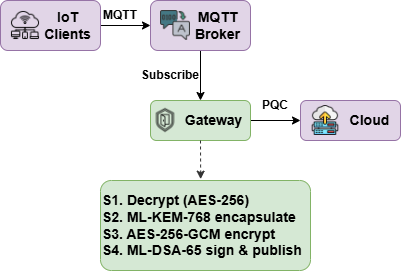
\includegraphics[width=0.95\columnwidth]{kics_image.png}
\caption{PQC payload translation pipeline. The gateway is a transparent quantum-safe upgrade boundary; device firmware is unmodified.}
\label{fig:pipeline}
\end{figure}

\subsection{Translation Steps}

For each received message payload $m$, the gateway executes:
\begin{enumerate}
  \item[\textbf{S1.}] \textbf{Decrypt:} Parse JSON and recover plaintext $p$ using the device's AES-256 key.
  \item[\textbf{S2.}] \textbf{KEM Encapsulate:} Call \texttt{ML-KEM-768.encap($pk_\text{cloud}$)} to obtain ciphertext $c_\text{kem}$ and shared secret $ss$; derive AES session key $k \leftarrow \text{HKDF}(ss)$.
  \item[\textbf{S3.}] \textbf{Encrypt:} Compute $c_\text{aes} \leftarrow \text{AES-256-GCM}_k(p,\,\eta)$ with a fresh 96-bit nonce $\eta$.
  \item[\textbf{S4.}] \textbf{Sign \& Publish:} Compute $\sigma \leftarrow \text{ML-DSA-65.sign}(c_\text{kem} \| c_\text{aes} \| \eta,\; sk_\text{gw})$ and forward $\{c_\text{kem}, c_\text{aes}, \eta, \sigma\}$ to the cloud.
\end{enumerate}
The prototype runs on a Raspberry Pi~4B (BCM2711 Cortex-A72, 4~GB LPDDR4) under Python~3.11 using \texttt{liboqs-python}~0.10~\cite{oqs2023}; per-stage latency is captured via \texttt{time.perf\_counter\_ns()} and written asynchronously to avoid timing perturbation.

\section{Experimental Evaluation}

\subsection{Setup}

Three IoT client profiles (AES-256-GCM only, Kyber-512+AES, and ML-KEM-768+ML-DSA-65) published 5~KB JSON payloads at 2-second intervals to a local Mosquitto~2.0 broker; the gateway processed 1,000~messages over a 20-minute window. Co-locating all components on the Raspberry Pi isolates PQC overhead from network variance; cloud-side decapsulation was omitted as commodity hardware processes it orders of magnitude faster.

\subsection{Processing Latency}

Table~\ref{tab:timing} reports per-stage wall-clock latency across all 1,000~messages.

\begin{table}[!t]
\centering
\captionsetup{font=footnotesize, skip=2pt}
\caption{Gateway PQC Processing Latency (Real liboqs, $N=1{,}000$)}
\label{tab:timing}
\footnotesize
\setlength{\tabcolsep}{3pt}
\begin{tabular}{lrrrrr}
\toprule
\textbf{Stage} & \textbf{Mean} & \textbf{Median} & \textbf{Std} & \textbf{P95} & \textbf{Max} \\
\midrule
ML-KEM-768 encap & 0.047 ms & 0.045 ms & 0.019 ms & 0.065 ms & 0.215 ms \\
AES-256 encrypt  & 0.030 ms & 0.018 ms & 0.143 ms & 0.024 ms & 1.609 ms \\
ML-DSA-65 sign   & 0.113 ms & 0.110 ms & 0.052 ms & 0.221 ms & 0.286 ms \\
\midrule
\textbf{Total}        & \textbf{0.189 ms} & \textbf{0.175 ms} & 0.176 ms & 0.297 ms & 1.979 ms \\
On-device handler     & 0.488 ms & 0.392 ms & 0.981 ms & 0.613 ms & 11.5 ms \\
\bottomrule
\end{tabular}
\vspace{-3mm}
\end{table}

ML-KEM-768 encapsulation averages 47~$\mu$s (std~19~$\mu$s), confirming lattice KEM efficiency on ARM Cortex-A72; ML-DSA-65 signing (113~$\mu$s) is the dominant cost. AES-256-GCM shows mean~$>$~P95 due to rare OS scheduling preemptions; the median of 18~$\mu$s reflects the typical fast path. Total P95 of 0.297~ms is negligible relative to any MQTT publish cadence; handler outliers (max~11.5~ms) reflect SBC jitter and warrant \texttt{PREEMPT\_RT} patching in production.

Our clients publish at 2-second intervals; the 0.297~ms P95 overhead consumes under 0.015\% of the publish budget, leaving ample single-core headroom even under concurrent device streams. The dominant cost is consequently the fixed cryptographic payload overhead analyzed below.

\subsection{Bandwidth Overhead}

The PQC overhead is a fixed 4,425 bytes per message regardless of payload size: ML-KEM-768 ciphertext (1,088~B), ML-DSA-65 signature (3,309~B), and AES-GCM nonce plus tag (28~B). With 5~KB payloads as used in our benchmarks, the gateway-to-cloud message is 9.4~KB (1.84$\times$ expansion). By confining translation to the gateway, the overhead is absorbed entirely by the high-capacity uplink while the constrained device link carries only the original small payload.

\subsection{Practical Viability}

These measurements confirm gateway-side PQC translation is production-ready on commodity ARM hardware. With combined ML-KEM-768 and ML-DSA-65 operations under 0.5~ms per message, gateways can easily parallelize concurrent streams. The 4,425-byte overhead is negligible for typical industrial deployments. Critically, this introduces NIST Level~3 security without modifying device firmware or existing infrastructure.

\section{Conclusion}

We measured a post-quantum MQTT gateway translation pipeline using ML-KEM-768 and ML-DSA-65 on Raspberry Pi~4B with real liboqs, achieving 0.189~ms mean latency across 1,000 messages. The fixed 4,425-byte PQC overhead expands 5~KB payloads to 9.4~KB on the gateway-to-cloud uplink, which easily absorbs it, validating NIST Level~3 PQC for IoT-to-cloud transit without modifying endpoint firmware. Future work will extend evaluation to distributed multi-Pi deployments and assess PREEMPT\_RT kernel patching for bounded handler latency.

\section*{Acknowledgment}
This work was supported in part by IITP (MSIT) under the Innovative Human Resource Development for Local Intellectualization (IITP-2025-RS-2020-II201612; 34\%) and the ITRC program (IITP-2025-RS-2024-00438430; 33\%), and by the NRF Basic Science Research Program (Ministry of Education, 2018R1A6A1A03024003; 33\%).
\balance

\begin{thebibliography}{9}

\bibitem{shor1994}
P.~W. Shor, ``Algorithms for quantum computation: Discrete logarithms and factoring,'' in \textit{Proc. 35th Annu. Symp. Foundations of Computer Science (FOCS)}, 1994, pp.~124--134.

\bibitem{mosca2018}
M.~Mosca, ``Cybersecurity in an era with quantum computers: Will we be ready?'' \textit{IEEE Secur. Privacy}, vol.~16, no.~5, pp.~38--41, 2018.

\bibitem{nist_fips203}
NIST, \textit{FIPS 203: Module-Lattice-Based Key-Encapsulation Mechanism Standard}, Gaithersburg, MD, 2024.

\bibitem{nist_fips204}
NIST, \textit{FIPS 204: Module-Lattice-Based Digital Signature Algorithm Standard}, Gaithersburg, MD, 2024.

\bibitem{oqs2023}
Open Quantum Safe Project, ``liboqs: Open-source quantum-safe cryptography library, v0.10,'' 2023. [Online]. Available: \url{https://openquantumsafe.org}

\end{thebibliography}

\end{document}
